% Options for packages loaded elsewhere
\PassOptionsToPackage{unicode}{hyperref}
\PassOptionsToPackage{hyphens}{url}
%
\documentclass[
]{article}
\usepackage{amsmath,amssymb}
\usepackage{lmodern}
\usepackage{iftex}
\ifPDFTeX
  \usepackage[T1]{fontenc}
  \usepackage[utf8]{inputenc}
  \usepackage{textcomp} % provide euro and other symbols
\else % if luatex or xetex
  \usepackage{unicode-math}
  \defaultfontfeatures{Scale=MatchLowercase}
  \defaultfontfeatures[\rmfamily]{Ligatures=TeX,Scale=1}
\fi
% Use upquote if available, for straight quotes in verbatim environments
\IfFileExists{upquote.sty}{\usepackage{upquote}}{}
\IfFileExists{microtype.sty}{% use microtype if available
  \usepackage[]{microtype}
  \UseMicrotypeSet[protrusion]{basicmath} % disable protrusion for tt fonts
}{}
\makeatletter
\@ifundefined{KOMAClassName}{% if non-KOMA class
  \IfFileExists{parskip.sty}{%
    \usepackage{parskip}
  }{% else
    \setlength{\parindent}{0pt}
    \setlength{\parskip}{6pt plus 2pt minus 1pt}}
}{% if KOMA class
  \KOMAoptions{parskip=half}}
\makeatother
\usepackage{xcolor}
\usepackage[margin=1in]{geometry}
\usepackage{color}
\usepackage{fancyvrb}
\newcommand{\VerbBar}{|}
\newcommand{\VERB}{\Verb[commandchars=\\\{\}]}
\DefineVerbatimEnvironment{Highlighting}{Verbatim}{commandchars=\\\{\}}
% Add ',fontsize=\small' for more characters per line
\usepackage{framed}
\definecolor{shadecolor}{RGB}{248,248,248}
\newenvironment{Shaded}{\begin{snugshade}}{\end{snugshade}}
\newcommand{\AlertTok}[1]{\textcolor[rgb]{0.94,0.16,0.16}{#1}}
\newcommand{\AnnotationTok}[1]{\textcolor[rgb]{0.56,0.35,0.01}{\textbf{\textit{#1}}}}
\newcommand{\AttributeTok}[1]{\textcolor[rgb]{0.77,0.63,0.00}{#1}}
\newcommand{\BaseNTok}[1]{\textcolor[rgb]{0.00,0.00,0.81}{#1}}
\newcommand{\BuiltInTok}[1]{#1}
\newcommand{\CharTok}[1]{\textcolor[rgb]{0.31,0.60,0.02}{#1}}
\newcommand{\CommentTok}[1]{\textcolor[rgb]{0.56,0.35,0.01}{\textit{#1}}}
\newcommand{\CommentVarTok}[1]{\textcolor[rgb]{0.56,0.35,0.01}{\textbf{\textit{#1}}}}
\newcommand{\ConstantTok}[1]{\textcolor[rgb]{0.00,0.00,0.00}{#1}}
\newcommand{\ControlFlowTok}[1]{\textcolor[rgb]{0.13,0.29,0.53}{\textbf{#1}}}
\newcommand{\DataTypeTok}[1]{\textcolor[rgb]{0.13,0.29,0.53}{#1}}
\newcommand{\DecValTok}[1]{\textcolor[rgb]{0.00,0.00,0.81}{#1}}
\newcommand{\DocumentationTok}[1]{\textcolor[rgb]{0.56,0.35,0.01}{\textbf{\textit{#1}}}}
\newcommand{\ErrorTok}[1]{\textcolor[rgb]{0.64,0.00,0.00}{\textbf{#1}}}
\newcommand{\ExtensionTok}[1]{#1}
\newcommand{\FloatTok}[1]{\textcolor[rgb]{0.00,0.00,0.81}{#1}}
\newcommand{\FunctionTok}[1]{\textcolor[rgb]{0.00,0.00,0.00}{#1}}
\newcommand{\ImportTok}[1]{#1}
\newcommand{\InformationTok}[1]{\textcolor[rgb]{0.56,0.35,0.01}{\textbf{\textit{#1}}}}
\newcommand{\KeywordTok}[1]{\textcolor[rgb]{0.13,0.29,0.53}{\textbf{#1}}}
\newcommand{\NormalTok}[1]{#1}
\newcommand{\OperatorTok}[1]{\textcolor[rgb]{0.81,0.36,0.00}{\textbf{#1}}}
\newcommand{\OtherTok}[1]{\textcolor[rgb]{0.56,0.35,0.01}{#1}}
\newcommand{\PreprocessorTok}[1]{\textcolor[rgb]{0.56,0.35,0.01}{\textit{#1}}}
\newcommand{\RegionMarkerTok}[1]{#1}
\newcommand{\SpecialCharTok}[1]{\textcolor[rgb]{0.00,0.00,0.00}{#1}}
\newcommand{\SpecialStringTok}[1]{\textcolor[rgb]{0.31,0.60,0.02}{#1}}
\newcommand{\StringTok}[1]{\textcolor[rgb]{0.31,0.60,0.02}{#1}}
\newcommand{\VariableTok}[1]{\textcolor[rgb]{0.00,0.00,0.00}{#1}}
\newcommand{\VerbatimStringTok}[1]{\textcolor[rgb]{0.31,0.60,0.02}{#1}}
\newcommand{\WarningTok}[1]{\textcolor[rgb]{0.56,0.35,0.01}{\textbf{\textit{#1}}}}
\usepackage{graphicx}
\makeatletter
\def\maxwidth{\ifdim\Gin@nat@width>\linewidth\linewidth\else\Gin@nat@width\fi}
\def\maxheight{\ifdim\Gin@nat@height>\textheight\textheight\else\Gin@nat@height\fi}
\makeatother
% Scale images if necessary, so that they will not overflow the page
% margins by default, and it is still possible to overwrite the defaults
% using explicit options in \includegraphics[width, height, ...]{}
\setkeys{Gin}{width=\maxwidth,height=\maxheight,keepaspectratio}
% Set default figure placement to htbp
\makeatletter
\def\fps@figure{htbp}
\makeatother
\setlength{\emergencystretch}{3em} % prevent overfull lines
\providecommand{\tightlist}{%
  \setlength{\itemsep}{0pt}\setlength{\parskip}{0pt}}
\setcounter{secnumdepth}{5}
\usepackage{float} \usepackage{graphicx} \floatplacement{figure}{H}
\ifLuaTeX
  \usepackage{selnolig}  % disable illegal ligatures
\fi
\IfFileExists{bookmark.sty}{\usepackage{bookmark}}{\usepackage{hyperref}}
\IfFileExists{xurl.sty}{\usepackage{xurl}}{} % add URL line breaks if available
\urlstyle{same} % disable monospaced font for URLs
\hypersetup{
  pdftitle={STA202 - Séries temporelles},
  pdfauthor={Anthony Kalaydjian - Mathieu Occhipinti},
  hidelinks,
  pdfcreator={LaTeX via pandoc}}

\title{STA202 - Séries temporelles}
\usepackage{etoolbox}
\makeatletter
\providecommand{\subtitle}[1]{% add subtitle to \maketitle
  \apptocmd{\@title}{\par {\large #1 \par}}{}{}
}
\makeatother
\subtitle{Rapport de projet}
\author{Anthony Kalaydjian - Mathieu Occhipinti}
\date{2023-03-02}

\begin{document}
\maketitle

\newpage
\thispagestyle{empty}

\mbox{}

\tableofcontents

\newpage
\thispagestyle{empty}

\mbox{}

\hypertarget{introduction}{%
\section{Introduction}\label{introduction}}

Au cours du dernier siècle, l'aggravation de la situation écologique a
conduit à une prise de conscience de l'importance de la qualité de
l'air. Ainsi, la concentration de certains gaz dans l'air a été étudiée
de manière approfondie afin de comprendre les effets de la pollution sur
l'environnement et la santé humaine. Les effets néfastes de la pollution
sont par exemple visibles auprès des joueurs d'échecs, dont les
performances diminuent lorsque la qualité de l'air de leur environnement
diminue.

On s'intérèsse ainsi, dans ce document, à l'étude de l'évolution de la
concentration de certains gaz dans l'air au cours du temps. Les données
que nous allons utiliser proviennent d'une banque de datasets mis à
disposition par l'université d'Irvine en Californie. Elles comportent
ainsi les mesures de la concentration de certains gaz dans une ville
d'Italie, sur une période de 1 an et avec un pas de 1h00.

\hypertarget{pruxe9traitement-et-mise-en-forme-des-donnuxe9es}{%
\section{Prétraitement et mise en forme des
données}\label{pruxe9traitement-et-mise-en-forme-des-donnuxe9es}}

\hypertarget{pruxe9traitement-et-gestion-des-donnuxe9es-manquantes}{%
\subsection{Prétraitement et gestion des données
manquantes}\label{pruxe9traitement-et-gestion-des-donnuxe9es-manquantes}}

Comme expliqué précédemment, les données que nous allons utiliser et qui
sont consignées dans un fichier .csv représentent l'évolution de la
concentration de certains gaz au cours du temps. Ces mesures sont en
fait des moyennes de ce qu'à mesuré le capteur sur 1h. Le dataset
présente également l'évolution de la température (en degrés Farenheit),
de l'humidité relative (en \%) ainsi que de l'humidité absolue. Toutes
ces données sont donc indéxées par la date et l'heure de la mesure.

Un premier problème est que certaines données sont manquantes. On peut
voir celà dans le dataset, où certaines valeurs associées à nos
variables vallent -200. Plusieurs techniques existent pour pallier ce
manque de données, dont le fait de ne pas prendre en compte les valeurs
manquantes ou bien de les remplacer par la moyenne des autres valeurs.
On effectuera cette dernière technique, qui semble mieux correspondre à
l'étude des séries temporelles. On évitera néanmoins les variables pour
lesquelles trop de données sont manquantes.

\begin{Shaded}
\begin{Highlighting}[]
\CommentTok{\# importation des données}
\NormalTok{air\_data }\OtherTok{\textless{}{-}} \FunctionTok{read.table}\NormalTok{(}\StringTok{"AirQualityUCI.csv"}\NormalTok{,}\AttributeTok{header=}\NormalTok{T,}\AttributeTok{sep=}\StringTok{";"}\NormalTok{)}

\CommentTok{\# resize}
\NormalTok{air\_data }\OtherTok{\textless{}{-}}\NormalTok{ air\_data[}\DecValTok{2}\SpecialCharTok{:}\DecValTok{9357}\NormalTok{,}\DecValTok{3}\SpecialCharTok{:}\DecValTok{15}\NormalTok{]}

\NormalTok{i }\OtherTok{\textless{}{-}} \FunctionTok{c}\NormalTok{(}\DecValTok{1}\SpecialCharTok{:}\FunctionTok{length}\NormalTok{(air\_data))}

\CommentTok{\# Remplacement des {-}200 par NA.}
\NormalTok{air\_data[, i] }\OtherTok{\textless{}{-}} \FunctionTok{apply}\NormalTok{(air\_data[, i], }\DecValTok{2}\NormalTok{, }\ControlFlowTok{function}\NormalTok{(x) (}\FunctionTok{gsub}\NormalTok{(}\SpecialCharTok{{-}}\DecValTok{200}\NormalTok{, }\ConstantTok{NA}\NormalTok{, x)))}

\CommentTok{\# Comptage du nombre de NA par colonne.}
\NormalTok{na\_count }\OtherTok{\textless{}{-}}\FunctionTok{sapply}\NormalTok{(air\_data, }\ControlFlowTok{function}\NormalTok{(y) }\FunctionTok{sum}\NormalTok{(}\FunctionTok{length}\NormalTok{(}\FunctionTok{which}\NormalTok{(}\FunctionTok{is.na}\NormalTok{(y)))))}

\CommentTok{\# Conversion des chaînes de caractère en nombres, en respectant la nomenclature française }
\CommentTok{\# des nombres à virgule.}
\NormalTok{air\_data[, i] }\OtherTok{\textless{}{-}} \FunctionTok{apply}\NormalTok{(air\_data[, i], }\DecValTok{2}\NormalTok{, }
                       \ControlFlowTok{function}\NormalTok{(x) }\FunctionTok{as.numeric}\NormalTok{(}\FunctionTok{as.character}\NormalTok{(}\FunctionTok{gsub}\NormalTok{(}\StringTok{","}\NormalTok{, }\StringTok{"."}\NormalTok{, x))))}

\CommentTok{\# Remplacement des NA par la moyenne.}
\NormalTok{air\_data[, i] }\OtherTok{\textless{}{-}} \FunctionTok{apply}\NormalTok{(air\_data[, i], }\DecValTok{2}\NormalTok{, }
                       \ControlFlowTok{function}\NormalTok{(x) }\FunctionTok{replace}\NormalTok{(x, }\FunctionTok{is.na}\NormalTok{(x), }\FunctionTok{mean}\NormalTok{(x, }\AttributeTok{na.rm =} \ConstantTok{TRUE}\NormalTok{)))}
\end{Highlighting}
\end{Shaded}

Les données sont bien du type floatant :

\begin{Shaded}
\begin{Highlighting}[]
\FunctionTok{str}\NormalTok{(air\_data)}
\end{Highlighting}
\end{Shaded}

\begin{verbatim}
## 'data.frame':    9356 obs. of  13 variables:
##  $ CO.GT.       : num  2 2.2 2.2 1.6 1.2 ...
##  $ PT08.S1.CO.  : num  1292 1402 1376 1272 1197 ...
##  $ NMHC.GT.     : num  112 88 80 51 38 31 31 24 19 14 ...
##  $ C6H6.GT.     : num  9.4 9 9.2 6.5 4.7 3.6 3.3 2.3 1.7 1.3 ...
##  $ PT08.S2.NMHC.: num  955 939 948 836 750 690 672 609 561 527 ...
##  $ NOx.GT.      : num  103 131 172 131 89 ...
##  $ PT08.S3.NOx. : num  1174 1140 1092 1205 1337 ...
##  $ NO2.GT.      : num  92 114 122 116 96 ...
##  $ PT08.S4.NO2. : num  1559 1555 1584 1490 1393 ...
##  $ PT08.S5.O3.  : num  972 1074 1203 1110 949 ...
##  $ T            : num  13.3 11.9 11 11.2 11.2 11.3 10.7 10.7 10.3 10.1 ...
##  $ RH           : num  47.7 54 60 59.6 59.2 56.8 60 59.7 60.2 60.5 ...
##  $ AH           : num  0.726 0.75 0.787 0.789 0.785 ...
\end{verbatim}

Les NA ont bien été remplacés :

\begin{Shaded}
\begin{Highlighting}[]
\FunctionTok{summary}\NormalTok{(air\_data)}
\end{Highlighting}
\end{Shaded}

\begin{verbatim}
##      CO.GT.        PT08.S1.CO.      NMHC.GT.         C6H6.GT.    
##  Min.   : 0.100   Min.   : 647   Min.   :   7.0   Min.   : 0.10  
##  1st Qu.: 1.200   1st Qu.: 941   1st Qu.: 218.9   1st Qu.: 4.60  
##  Median : 2.153   Median :1075   Median : 218.9   Median : 8.60  
##  Mean   : 2.153   Mean   :1100   Mean   : 218.9   Mean   :10.08  
##  3rd Qu.: 2.600   3rd Qu.:1221   3rd Qu.: 218.9   3rd Qu.:13.60  
##  Max.   :11.900   Max.   :2040   Max.   :1189.0   Max.   :63.70  
##  PT08.S2.NMHC.       NOx.GT.        PT08.S3.NOx.       NO2.GT.     
##  Min.   : 383.0   Min.   :   2.0   Min.   : 322.0   Min.   :  2.0  
##  1st Qu.: 742.8   1st Qu.: 112.0   1st Qu.: 666.0   1st Qu.: 86.0  
##  Median : 923.0   Median : 229.0   Median : 818.0   Median :113.1  
##  Mean   : 939.1   Mean   : 246.9   Mean   : 835.5   Mean   :113.1  
##  3rd Qu.:1105.0   3rd Qu.: 284.0   3rd Qu.: 960.0   3rd Qu.:133.0  
##  Max.   :2214.0   Max.   :1479.0   Max.   :2683.0   Max.   :340.0  
##   PT08.S4.NO2.   PT08.S5.O3.         T               RH              AH        
##  Min.   : 551   Min.   : 221   Min.   :-1.90   Min.   : 9.20   Min.   :0.1847  
##  1st Qu.:1242   1st Qu.: 742   1st Qu.:12.00   1st Qu.:36.60   1st Qu.:0.7460  
##  Median :1456   Median : 983   Median :18.30   Median :49.23   Median :1.0154  
##  Mean   :1456   Mean   :1023   Mean   :18.32   Mean   :49.23   Mean   :1.0256  
##  3rd Qu.:1662   3rd Qu.:1255   3rd Qu.:24.10   3rd Qu.:61.90   3rd Qu.:1.2963  
##  Max.   :2775   Max.   :2523   Max.   :44.60   Max.   :88.70   Max.   :2.2310
\end{verbatim}

Sur l'ensemble des données que l'on a, on peut voir qu'il manque
beaucoup de données pour les gaz CO.GT, NMHC.GT, NOx.GT et NO2.GT avec
respectivement 1683, 8444, 1640 et 1643 données manquantes sur un total
de 9357 valeurs. On évitera ainsi de porter l'étude sur ces données.
Pour les autres colonnes, il ne nous manque que 366 ou 367 valeurs, ce
qui représente 4\% des valeurs. Ce n'est pas parfait, mais suffisamment
raisonnable pour mener l'étude. Ces valeurs manquantes peuvent être dues
à des pannes générales du capteur, qui ont provoqué le même nombre de
valeurs manquantes pour chaque colonne.

\begin{Shaded}
\begin{Highlighting}[]
\FunctionTok{print}\NormalTok{(na\_count)}
\end{Highlighting}
\end{Shaded}

\begin{verbatim}
##        CO.GT.   PT08.S1.CO.      NMHC.GT.      C6H6.GT. PT08.S2.NMHC. 
##          1683           366          8443           366           366 
##       NOx.GT.  PT08.S3.NOx.       NO2.GT.  PT08.S4.NO2.   PT08.S5.O3. 
##          1639           366          1642           366           366 
##             T            RH            AH 
##           366           366           366
\end{verbatim}

Les séries que nous allons étudier sont donc les suivantes :\newline
PT08.CO, C6H6.GT, PT08.NMHC, PT08.NOx, PT08.NO2 et PT08.O3.

\begin{Shaded}
\begin{Highlighting}[]
\NormalTok{air\_data }\OtherTok{\textless{}{-}}\NormalTok{ air\_data[, }\SpecialCharTok{{-}}\FunctionTok{c}\NormalTok{(}\DecValTok{1}\NormalTok{, }\DecValTok{3}\NormalTok{, }\DecValTok{5}\NormalTok{, }\DecValTok{7}\NormalTok{)]}
\end{Highlighting}
\end{Shaded}

\hypertarget{cruxe9ation-des-suxe9ries-temporelles}{%
\subsection{Création des séries
temporelles}\label{cruxe9ation-des-suxe9ries-temporelles}}

\begin{Shaded}
\begin{Highlighting}[]
\NormalTok{date1 }\OtherTok{\textless{}{-}} \FunctionTok{strptime}\NormalTok{(}\StringTok{"03/10/2004 18:00:00"}\NormalTok{, }\StringTok{"\%m/\%d/\%Y \%H:\%M:\%S"}\NormalTok{)}
\NormalTok{date2 }\OtherTok{\textless{}{-}} \FunctionTok{strptime}\NormalTok{(}\StringTok{"04/04/2005 14:00:00"}\NormalTok{, }\StringTok{"\%m/\%d/\%Y \%H:\%M:\%S"}\NormalTok{)}
\NormalTok{Date\_air }\OtherTok{\textless{}{-}} \FunctionTok{seq.POSIXt}\NormalTok{(date1,date2, }\AttributeTok{by =} \StringTok{"1 hour"}\NormalTok{)}

\NormalTok{ts\_PT08.CO }\OtherTok{\textless{}{-}} \FunctionTok{xts}\NormalTok{(air\_data}\SpecialCharTok{$}\NormalTok{PT08.S1.CO., }\AttributeTok{order.by=}\NormalTok{Date\_air)}
\NormalTok{ts\_C6H6.GT }\OtherTok{\textless{}{-}} \FunctionTok{xts}\NormalTok{(air\_data}\SpecialCharTok{$}\NormalTok{C6H6.GT., }\AttributeTok{order.by=}\NormalTok{Date\_air)}
\NormalTok{ts\_PT08.NMHC }\OtherTok{\textless{}{-}} \FunctionTok{xts}\NormalTok{(air\_data}\SpecialCharTok{$}\NormalTok{PT08.S2.NMHC., }\AttributeTok{order.by=}\NormalTok{Date\_air)}
\NormalTok{ts\_PT08.NOx }\OtherTok{\textless{}{-}} \FunctionTok{xts}\NormalTok{(air\_data}\SpecialCharTok{$}\NormalTok{PT08.S3.NOx., }\AttributeTok{order.by=}\NormalTok{Date\_air)}
\NormalTok{ts\_PT08.NO2 }\OtherTok{\textless{}{-}} \FunctionTok{xts}\NormalTok{(air\_data}\SpecialCharTok{$}\NormalTok{PT08.S4.NO2.,}\AttributeTok{order.by=}\NormalTok{Date\_air)}
\NormalTok{ts\_PT08.O3 }\OtherTok{\textless{}{-}} \FunctionTok{xts}\NormalTok{(air\_data}\SpecialCharTok{$}\NormalTok{PT08.S5.O3.,}\AttributeTok{order.by=}\NormalTok{Date\_air)}
\end{Highlighting}
\end{Shaded}

\hypertarget{analyse-descriptive-des-donnuxe9es}{%
\section{Analyse descriptive des
données}\label{analyse-descriptive-des-donnuxe9es}}

\hypertarget{corruxe9lation-des-variables-observuxe9es}{%
\subsection{Corrélation des variables
observées}\label{corruxe9lation-des-variables-observuxe9es}}

La figure \ref{fig:figs} montre la matrice de correlation de nos
variables. Elle montre ainsi que la température et l'humidité absolue ne
sont visiblement corrélées qu'avec les émissions de NO2(GT). Hormis
cela, aucun des trois paramètres que sont la température, l'humidité
relative et l'humidité absolue ne semble être corrélés avec les
concentrations de gaz mesurés dans l'air. Cette matrice nous montre
également une forte corrélation positive entre les autres gaz, ce qui
peut montrer que leur comportement est similaire.

\begin{figure}

{\centering \includegraphics{STA202_report_files/figure-latex/figs-1} 

}

\caption{\label{fig:figs}Matrice de corrélation des variables observées}\label{fig:figs}
\end{figure}

\hypertarget{analyse-en-suxe9rie-temporelle}{%
\subsection{Analyse en série
temporelle}\label{analyse-en-suxe9rie-temporelle}}

L'observation des différentes concentration moyennes périodiques, ainsi
que des séries temporelles elles-mêmes montre un comportement très
similaires entre l'ensemble des gas, si ce n'est pour le Nox.GT dont le
comportement varie. Les émissions hebdomadaires semblent ainsi
inversées, avec un pic d'émissions les lundis et dimanches contre des
pics d'émission en milieu de semaine pour les autres gas. Il en est de
même pour les émissions horaires, avec plus d'émissions tôt le matin
(vers 5h) contre des émissions plus présentes au milieu de la journée
avec les autres gas. Ceci pourrait être expliqué par le fait que les
émissions de ce gaz soient majoritairement dues aux émissions de
transports. Ainsi, les livraisons des magasins par les camions
transporteurs, qui se font en début de semaine et tôt le matin, peuvent
expliquer ces émissions différentes.

\begin{figure}

{\centering \includegraphics{STA202_report_files/figure-latex/PT08.CO-1} 

}

\caption{\label{fig:PT08.CO} Concentrations moyennes périodiques PT08.CO}\label{fig:PT08.CO}
\end{figure}

\begin{figure}
  \centering
  \includegraphics[height=3cm]{Nox}
  \caption{Concentrations moyennes périodiques NOx.GT}
\end{figure}

La plupart des gaz ayant un comportement similaire, on choisira par la
suite de ne travailler que sur la série temporelle associée à la
concentration de PT08.CO.

\hypertarget{moduxe9lisation-des-donnuxe9es}{%
\section{Modélisation des
données}\label{moduxe9lisation-des-donnuxe9es}}

\hypertarget{tendances}{%
\subsection{Tendances}\label{tendances}}

L'analyse de la tendance de la série temporelle peut être faite à l'aide
de la moyenne mobile. Un modèle approprié doit pouvoir faire abstraction
du cycle journalier des données. Pour ce faire nous allons utiliser la
fonction movavg de la librairie pracma. Nous allons passer comme
argument n=720 : le nombre de points que l'on regarde avant pour prédire
la suite (cela correspond à un moins dans notre cas d'étude). Le second
argument est le type de moyenne mobile, nous avons choisi `w' pour
weighted. Cela signifie que plus le point est éloigné de notre point de
prédiction, plus son poids dans le calcul de la moyenne mobile est
faible. La décroissance des poids est linéaire. Voici, la tendance de
notre série chronologique obtenue.

\begin{Shaded}
\begin{Highlighting}[]
\NormalTok{MA}\OtherTok{\textless{}{-}}\FunctionTok{movavg}\NormalTok{(ts\_PT08.CO,}\AttributeTok{n=}\DecValTok{720}\NormalTok{,}\AttributeTok{type=}\StringTok{\textquotesingle{}w\textquotesingle{}}\NormalTok{)}
\NormalTok{MA}\OtherTok{\textless{}{-}}\FunctionTok{xts}\NormalTok{(MA,}\AttributeTok{order.by=}\NormalTok{Date\_air)}
\FunctionTok{plot}\NormalTok{(ts\_PT08.CO)}
\end{Highlighting}
\end{Shaded}

\includegraphics{STA202_report_files/figure-latex/unnamed-chunk-7-1.pdf}

\begin{Shaded}
\begin{Highlighting}[]
\FunctionTok{lines}\NormalTok{(MA,}\AttributeTok{col=}\StringTok{\textquotesingle{}red\textquotesingle{}}\NormalTok{,}\AttributeTok{type=}\StringTok{\textquotesingle{}l\textquotesingle{}}\NormalTok{)}
\end{Highlighting}
\end{Shaded}

\includegraphics{STA202_report_files/figure-latex/unnamed-chunk-7-2.pdf}

\hypertarget{saisonnalituxe9}{%
\subsection{Saisonnalité}\label{saisonnalituxe9}}

Pour étudier la saisonnalité de nos données nous allons regarder
l'autocorélogramme de notre série.

\begin{Shaded}
\begin{Highlighting}[]
\FunctionTok{Acf}\NormalTok{(ts\_PT08.CO,}\AttributeTok{lag.max=}\DecValTok{500}\NormalTok{)}
\end{Highlighting}
\end{Shaded}

\includegraphics{STA202_report_files/figure-latex/unnamed-chunk-8-1.pdf}

L'oscillation de l'ACF avec des pics réguliers toutes les 24h (et même
12h) montre l'existence d'une saisonnalité journalière dans nos données.
L'existance de cette saisonnalité dément la stationnarité de la série
temporelle. Ceci peut également être vérifié en utilisant le test KPSS
(Kwiatkowski--Phillips--Schmidt--Shin), qui teste l'hypothèse nulle
suivante : \[(H_0): \text{La série temporelle est stationnaire}\] Le
test KPSS affiche une valeur de test de 1.1339, ce qui est bien au
dessus de toutes les valeurs critiques. On rejette ainsi l'hypothèse
nulle. La série temporelle n'est donc pas stationnaire.

\begin{Shaded}
\begin{Highlighting}[]
\FunctionTok{ur.kpss}\NormalTok{(ts\_PT08.CO) }\SpecialCharTok{\%\textgreater{}\%}
  \FunctionTok{summary}\NormalTok{()}
\end{Highlighting}
\end{Shaded}

\begin{verbatim}
## 
## ####################### 
## # KPSS Unit Root Test # 
## ####################### 
## 
## Test is of type: mu with 12 lags. 
## 
## Value of test-statistic is: 1.134 
## 
## Critical value for a significance level of: 
##                 10pct  5pct 2.5pct  1pct
## critical values 0.347 0.463  0.574 0.739
\end{verbatim}

La stationnarité va pouvoir être atteinte en différenciant la série
temporelle. La saisonnalité journalière nous pousse ainsi à différencier
nos données avec un lag de 24 via l'opérateur \(1-L^{24}\). Nous
affichons maintenant l'autocorrélogramme de notre série différenciée :

\begin{Shaded}
\begin{Highlighting}[]
\NormalTok{CO.diff}\OtherTok{\textless{}{-}}\FunctionTok{na\_mean}\NormalTok{(}\FunctionTok{diff}\NormalTok{(ts\_PT08.CO,}\AttributeTok{lag=}\DecValTok{24}\NormalTok{,}\AttributeTok{differences=}\DecValTok{1}\NormalTok{))}

\FunctionTok{Acf}\NormalTok{(CO.diff,}\AttributeTok{lag.max=}\DecValTok{2000}\NormalTok{)}
\end{Highlighting}
\end{Shaded}

\includegraphics{STA202_report_files/figure-latex/unnamed-chunk-9-1.pdf}

On obtient un graphique satisfaisant avec une décroissance exponentielle
vers zéro. On souhaite maintenant déduire les plages de paramètres
possibles pour un modèle SARIMA, (p,P,q,Q). Pour ce faire, on étudie
l'autocorrélogramme et l'autocorrélogramme partiel de la série
différenciée.

\begin{Shaded}
\begin{Highlighting}[]
\FunctionTok{Acf}\NormalTok{(CO.diff,}\AttributeTok{lag.max=}\DecValTok{100}\NormalTok{)}
\end{Highlighting}
\end{Shaded}

\includegraphics{STA202_report_files/figure-latex/unnamed-chunk-10-1.pdf}

\begin{Shaded}
\begin{Highlighting}[]
\FunctionTok{Pacf}\NormalTok{(CO.diff,}\AttributeTok{lag=}\DecValTok{100}\NormalTok{)}
\end{Highlighting}
\end{Shaded}

\includegraphics{STA202_report_files/figure-latex/unnamed-chunk-10-2.pdf}
\#\# Partie aléatoire \#\# Stationnarité

\hypertarget{simulation}{%
\section{Simulation}\label{simulation}}

\begin{Shaded}
\begin{Highlighting}[]
\CommentTok{\# kernel}
\NormalTok{X}\OtherTok{\textless{}{-}}\NormalTok{(air\_data}\SpecialCharTok{$}\NormalTok{PT08.S1.CO. }\SpecialCharTok{{-}} \FunctionTok{mean}\NormalTok{(air\_data}\SpecialCharTok{$}\NormalTok{PT08.S1.CO.))}\SpecialCharTok{/}\FunctionTok{sd}\NormalTok{(air\_data}\SpecialCharTok{$}\NormalTok{PT08.S1.CO.)}

\FunctionTok{head}\NormalTok{(X)}
\end{Highlighting}
\end{Shaded}

\begin{verbatim}
## [1] 0.9032349 1.4201861 1.2979976 0.8092437 0.4567770 0.4003823
\end{verbatim}

\begin{Shaded}
\begin{Highlighting}[]
\NormalTok{X}\OtherTok{\textless{}{-}}\FunctionTok{xts}\NormalTok{(X,}\AttributeTok{order.by=}\NormalTok{Date\_air)}
\NormalTok{n }\OtherTok{\textless{}{-}} \FunctionTok{length}\NormalTok{(Date\_air)}
\NormalTok{t }\OtherTok{\textless{}{-}} \FunctionTok{c}\NormalTok{(}\DecValTok{1}\SpecialCharTok{:}\NormalTok{n)}
\NormalTok{h}\OtherTok{\textless{}{-}}\DecValTok{2000}
\CommentTok{\#h \textless{}{-} 100}
\NormalTok{x}\OtherTok{\textless{}{-}}\FunctionTok{seq}\NormalTok{(}\DecValTok{1}\NormalTok{,}\FunctionTok{max}\NormalTok{(t),}\AttributeTok{length=}\NormalTok{n)}
\CommentTok{\# test\textless{}{-}lapply(x,function(x)\{x\^{}2\})}
\CommentTok{\# test[[1]]}
\CommentTok{\# test}
\NormalTok{noyau }\OtherTok{\textless{}{-}} \ControlFlowTok{function}\NormalTok{(x)\{}\FunctionTok{dnorm}\NormalTok{(x}\SpecialCharTok{{-}}\NormalTok{t,}\DecValTok{0}\NormalTok{,}\AttributeTok{sd=}\FunctionTok{sqrt}\NormalTok{(h}\SpecialCharTok{/}\DecValTok{2}\NormalTok{))}\SpecialCharTok{/}\FunctionTok{sum}\NormalTok{(}\FunctionTok{dnorm}\NormalTok{(x}\SpecialCharTok{{-}}\NormalTok{t,}\DecValTok{0}\NormalTok{,}\AttributeTok{sd=}\FunctionTok{sqrt}\NormalTok{(h}\SpecialCharTok{/}\DecValTok{2}\NormalTok{)))\}}

\NormalTok{W}\OtherTok{\textless{}{-}}\FunctionTok{matrix}\NormalTok{(}\FunctionTok{unlist}\NormalTok{(}\FunctionTok{lapply}\NormalTok{(x,noyau)),}\AttributeTok{ncol=}\NormalTok{n,}\AttributeTok{nrow=}\NormalTok{n,}\AttributeTok{byrow=}\NormalTok{F)}

\FunctionTok{plot}\NormalTok{(W[,}\DecValTok{1}\NormalTok{], }\AttributeTok{type=}\StringTok{\textquotesingle{}l\textquotesingle{}}\NormalTok{)}
\end{Highlighting}
\end{Shaded}

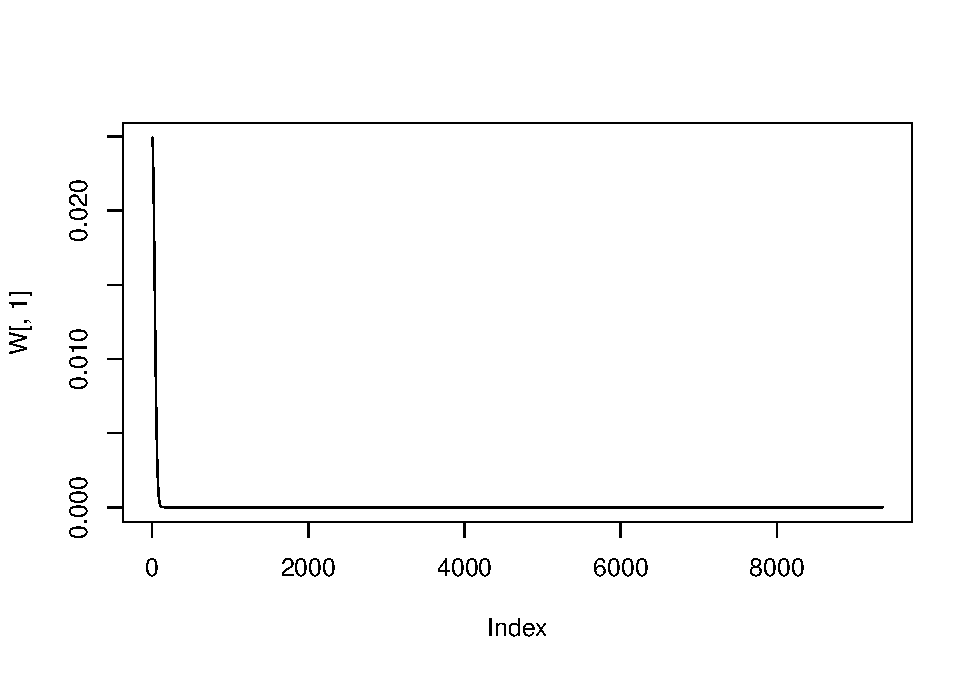
\includegraphics{STA202_report_files/figure-latex/tests-1.pdf}

\begin{Shaded}
\begin{Highlighting}[]
\NormalTok{ychap.kernel}\OtherTok{\textless{}{-}}\FunctionTok{colSums}\NormalTok{(}\FunctionTok{as.numeric}\NormalTok{(X)}\SpecialCharTok{*}\NormalTok{W)}
\NormalTok{ychap.kernel}\OtherTok{\textless{}{-}}\FunctionTok{xts}\NormalTok{(ychap.kernel,}\AttributeTok{order.by=}\NormalTok{Date\_air)}
\FunctionTok{plot}\NormalTok{(X,}\AttributeTok{type=}\StringTok{\textquotesingle{}l\textquotesingle{}}\NormalTok{)}
\end{Highlighting}
\end{Shaded}

\includegraphics{STA202_report_files/figure-latex/tests-2.pdf}

\begin{Shaded}
\begin{Highlighting}[]
\FunctionTok{lines}\NormalTok{(ychap.kernel,}\AttributeTok{col=}\StringTok{\textquotesingle{}red\textquotesingle{}}\NormalTok{)}
\end{Highlighting}
\end{Shaded}

\includegraphics{STA202_report_files/figure-latex/tests-3.pdf}

\begin{Shaded}
\begin{Highlighting}[]
\CommentTok{\#Normalization}
\NormalTok{X}\OtherTok{=}\NormalTok{ (ts\_PT08.CO }\SpecialCharTok{{-}} \FunctionTok{mean}\NormalTok{(air\_data}\SpecialCharTok{$}\NormalTok{PT08.S1.CO.))}\SpecialCharTok{/}\FunctionTok{sd}\NormalTok{(ts\_PT08.CO)}
\FunctionTok{plot}\NormalTok{(X)}
\end{Highlighting}
\end{Shaded}

\includegraphics{STA202_report_files/figure-latex/unnamed-chunk-11-1.pdf}

\begin{Shaded}
\begin{Highlighting}[]
\FunctionTok{plot}\NormalTok{(ts\_PT08.CO)}
\end{Highlighting}
\end{Shaded}

\includegraphics{STA202_report_files/figure-latex/unnamed-chunk-11-2.pdf}

\begin{Shaded}
\begin{Highlighting}[]
\FunctionTok{dygraph}\NormalTok{(X) }\SpecialCharTok{\%\textgreater{}\%} \FunctionTok{dyRangeSelector}\NormalTok{()}
\end{Highlighting}
\end{Shaded}

\begin{Shaded}
\begin{Highlighting}[]
\CommentTok{\# Trend modelisation using a quadratic function}
\NormalTok{t }\OtherTok{\textless{}{-}} \FunctionTok{c}\NormalTok{(}\DecValTok{1}\SpecialCharTok{:}\FunctionTok{length}\NormalTok{(Date\_air))}
\NormalTok{reg}\OtherTok{\textless{}{-}}\FunctionTok{lm}\NormalTok{(X}\SpecialCharTok{\textasciitilde{}}\NormalTok{t}\SpecialCharTok{+}\FunctionTok{I}\NormalTok{(t}\SpecialCharTok{\^{}}\DecValTok{2}\NormalTok{))}
\NormalTok{y.chap.lm }\OtherTok{\textless{}{-}} \FunctionTok{xts}\NormalTok{(reg}\SpecialCharTok{$}\NormalTok{fitted, }\AttributeTok{order.by =}\NormalTok{ Date\_air)}
\FunctionTok{lines}\NormalTok{(y.chap.lm, }\AttributeTok{col=}\StringTok{\textquotesingle{}red\textquotesingle{}}\NormalTok{)}
\end{Highlighting}
\end{Shaded}

\includegraphics{STA202_report_files/figure-latex/unnamed-chunk-11-4.pdf}

\begin{Shaded}
\begin{Highlighting}[]
\FunctionTok{plot}\NormalTok{(X}\SpecialCharTok{{-}}\NormalTok{y.chap.lm)  }
\end{Highlighting}
\end{Shaded}

\includegraphics{STA202_report_files/figure-latex/unnamed-chunk-11-5.pdf}

\begin{Shaded}
\begin{Highlighting}[]
\CommentTok{\# Trend modelisation using Moving average trend}
\NormalTok{l }\OtherTok{\textless{}{-}} \DecValTok{24}
\NormalTok{mb }\OtherTok{\textless{}{-}}\NormalTok{ stats}\SpecialCharTok{::}\FunctionTok{filter}\NormalTok{(X, }\AttributeTok{filter=}\FunctionTok{array}\NormalTok{(}\DecValTok{1}\SpecialCharTok{/}\NormalTok{l,}\AttributeTok{dim=}\NormalTok{l),}
                  \AttributeTok{method =} \FunctionTok{c}\NormalTok{(}\StringTok{"convolution"}\NormalTok{),}
                  \AttributeTok{sides =} \DecValTok{2}\NormalTok{, }\AttributeTok{circular =}\NormalTok{ F)}
\NormalTok{mb }\OtherTok{\textless{}{-}} \FunctionTok{xts}\NormalTok{(mb,}\AttributeTok{order.by=}\NormalTok{Date\_air)}
\NormalTok{X.detrend }\OtherTok{\textless{}{-}}\NormalTok{ X }\SpecialCharTok{{-}}\NormalTok{ mb}
\FunctionTok{plot}\NormalTok{(X)}
\end{Highlighting}
\end{Shaded}

\includegraphics{STA202_report_files/figure-latex/unnamed-chunk-11-6.pdf}

\begin{Shaded}
\begin{Highlighting}[]
\FunctionTok{lines}\NormalTok{(mb, }\AttributeTok{col=}\StringTok{\textquotesingle{}red\textquotesingle{}}\NormalTok{)}
\end{Highlighting}
\end{Shaded}

\includegraphics{STA202_report_files/figure-latex/unnamed-chunk-11-7.pdf}

\begin{Shaded}
\begin{Highlighting}[]
\FunctionTok{lines}\NormalTok{(X.detrend, }\AttributeTok{col=}\StringTok{\textquotesingle{}green\textquotesingle{}}\NormalTok{)}
\end{Highlighting}
\end{Shaded}

\includegraphics{STA202_report_files/figure-latex/unnamed-chunk-11-8.pdf}

\begin{Shaded}
\begin{Highlighting}[]
\FunctionTok{dygraph}\NormalTok{(X.detrend) }\SpecialCharTok{\%\textgreater{}\%} \FunctionTok{dyRangeSelector}\NormalTok{()}
\end{Highlighting}
\end{Shaded}

\begin{Shaded}
\begin{Highlighting}[]
\CommentTok{\#Seasonality}
\DocumentationTok{\#\#\# A FAIRE }\AlertTok{\#\#\#}



\CommentTok{\# }\AlertTok{TEST}\CommentTok{ Auto decompose}
\FunctionTok{Acf}\NormalTok{(X, }\AttributeTok{lag.max=}\DecValTok{1000}\NormalTok{)}
\end{Highlighting}
\end{Shaded}

\includegraphics{STA202_report_files/figure-latex/unnamed-chunk-11-10.pdf}

\begin{Shaded}
\begin{Highlighting}[]
\NormalTok{X.diff }\OtherTok{\textless{}{-}} \FunctionTok{diff}\NormalTok{(X, }\AttributeTok{lag =} \DecValTok{24}\NormalTok{, }\AttributeTok{difference=}\DecValTok{2}\NormalTok{)}
\FunctionTok{Acf}\NormalTok{(X.diff, }\AttributeTok{lag.max=}\DecValTok{1000}\NormalTok{)}
\end{Highlighting}
\end{Shaded}

\includegraphics{STA202_report_files/figure-latex/unnamed-chunk-11-11.pdf}

\begin{Shaded}
\begin{Highlighting}[]
\NormalTok{X.decompose }\OtherTok{\textless{}{-}} \FunctionTok{decompose}\NormalTok{(}\FunctionTok{ts}\NormalTok{(X.diff, }\AttributeTok{frequency=}\DecValTok{24}\NormalTok{))}
\FunctionTok{plot}\NormalTok{(X.decompose}\SpecialCharTok{$}\NormalTok{x)}
\FunctionTok{lines}\NormalTok{(X.decompose}\SpecialCharTok{$}\NormalTok{trend, }\AttributeTok{col=}\StringTok{\textquotesingle{}red\textquotesingle{}}\NormalTok{)}
\end{Highlighting}
\end{Shaded}

\includegraphics{STA202_report_files/figure-latex/unnamed-chunk-11-12.pdf}

\begin{Shaded}
\begin{Highlighting}[]
\FunctionTok{plot}\NormalTok{(X.decompose}\SpecialCharTok{$}\NormalTok{seasonal, }\AttributeTok{col=}\StringTok{\textquotesingle{}blue\textquotesingle{}}\NormalTok{)}
\end{Highlighting}
\end{Shaded}

\includegraphics{STA202_report_files/figure-latex/unnamed-chunk-11-13.pdf}

\begin{Shaded}
\begin{Highlighting}[]
\FunctionTok{plot}\NormalTok{(X.decompose}\SpecialCharTok{$}\NormalTok{random)}
\end{Highlighting}
\end{Shaded}

\includegraphics{STA202_report_files/figure-latex/unnamed-chunk-11-14.pdf}

\begin{Shaded}
\begin{Highlighting}[]
\FunctionTok{Acf}\NormalTok{(X.decompose}\SpecialCharTok{$}\NormalTok{random)}
\end{Highlighting}
\end{Shaded}

\includegraphics{STA202_report_files/figure-latex/unnamed-chunk-11-15.pdf}

\begin{Shaded}
\begin{Highlighting}[]
\CommentTok{\# modélisation du résidu}
\NormalTok{residual }\OtherTok{=}\NormalTok{ X.decompose}\SpecialCharTok{$}\NormalTok{random}
\NormalTok{residual }\OtherTok{\textless{}{-}} \FunctionTok{apply}\NormalTok{(residual, }\DecValTok{2}\NormalTok{, }
                  \ControlFlowTok{function}\NormalTok{(x) }\FunctionTok{replace}\NormalTok{(x, }\FunctionTok{is.na}\NormalTok{(x), }\FunctionTok{mean}\NormalTok{(x, }\AttributeTok{na.rm =} \ConstantTok{TRUE}\NormalTok{)))}

\FunctionTok{Acf}\NormalTok{(residual, }\AttributeTok{lag.max=}\DecValTok{50}\NormalTok{)}
\end{Highlighting}
\end{Shaded}

\includegraphics{STA202_report_files/figure-latex/unnamed-chunk-11-16.pdf}

\begin{Shaded}
\begin{Highlighting}[]
\FunctionTok{Pacf}\NormalTok{(residual, }\AttributeTok{lag.max=}\DecValTok{50}\NormalTok{)}
\end{Highlighting}
\end{Shaded}

\includegraphics{STA202_report_files/figure-latex/unnamed-chunk-11-17.pdf}

\begin{Shaded}
\begin{Highlighting}[]
\NormalTok{residual.model }\OtherTok{\textless{}{-}} \FunctionTok{auto.arima}\NormalTok{(residual)}
\FunctionTok{summary}\NormalTok{(residual.model)}
\end{Highlighting}
\end{Shaded}

\begin{verbatim}
## Series: residual 
## ARIMA(5,0,0) with zero mean 
## 
## Coefficients:
##          ar1      ar2     ar3      ar4      ar5
##       0.7187  -0.1336  0.0354  -0.0614  -0.0731
## s.e.  0.0103   0.0127  0.0128   0.0127   0.0103
## 
## sigma^2 = 0.553:  log likelihood = -10502.37
## AIC=21016.74   AICc=21016.75   BIC=21059.6
## 
## Training set error measures:
##                         ME      RMSE       MAE      MPE     MAPE      MASE
## Training set -0.0004173901 0.7434557 0.5440593 97.47243 354.0662 0.8957985
##                      ACF1
## Training set -0.005648761
\end{verbatim}

\begin{Shaded}
\begin{Highlighting}[]
\FunctionTok{plot}\NormalTok{(residual.model}\SpecialCharTok{$}\NormalTok{residuals)}
\end{Highlighting}
\end{Shaded}

\includegraphics{STA202_report_files/figure-latex/unnamed-chunk-11-18.pdf}

\begin{Shaded}
\begin{Highlighting}[]
\FunctionTok{adf.test}\NormalTok{(residual.model}\SpecialCharTok{$}\NormalTok{residuals)}
\end{Highlighting}
\end{Shaded}

\begin{verbatim}
## Augmented Dickey-Fuller Test 
## alternative: stationary 
##  
## Type 1: no drift no trend 
##       lag   ADF p.value
##  [1,]   0 -97.3    0.01
##  [2,]   1 -69.7    0.01
##  [3,]   2 -57.8    0.01
##  [4,]   3 -51.2    0.01
##  [5,]   4 -44.5    0.01
##  [6,]   5 -40.5    0.01
##  [7,]   6 -39.0    0.01
##  [8,]   7 -39.4    0.01
##  [9,]   8 -39.1    0.01
## [10,]   9 -40.1    0.01
## [11,]  10 -40.6    0.01
## Type 2: with drift no trend 
##       lag   ADF p.value
##  [1,]   0 -97.3    0.01
##  [2,]   1 -69.7    0.01
##  [3,]   2 -57.8    0.01
##  [4,]   3 -51.2    0.01
##  [5,]   4 -44.5    0.01
##  [6,]   5 -40.5    0.01
##  [7,]   6 -39.0    0.01
##  [8,]   7 -39.4    0.01
##  [9,]   8 -39.1    0.01
## [10,]   9 -40.1    0.01
## [11,]  10 -40.6    0.01
## Type 3: with drift and trend 
##       lag   ADF p.value
##  [1,]   0 -97.3    0.01
##  [2,]   1 -69.7    0.01
##  [3,]   2 -57.8    0.01
##  [4,]   3 -51.2    0.01
##  [5,]   4 -44.5    0.01
##  [6,]   5 -40.5    0.01
##  [7,]   6 -39.0    0.01
##  [8,]   7 -39.4    0.01
##  [9,]   8 -39.1    0.01
## [10,]   9 -40.1    0.01
## [11,]  10 -40.6    0.01
## ---- 
## Note: in fact, p.value = 0.01 means p.value <= 0.01
\end{verbatim}

\begin{Shaded}
\begin{Highlighting}[]
\FunctionTok{shapiro.test}\NormalTok{(residual.model}\SpecialCharTok{$}\NormalTok{residuals[}\FunctionTok{c}\NormalTok{(}\DecValTok{1}\SpecialCharTok{:}\DecValTok{5000}\NormalTok{)])}
\end{Highlighting}
\end{Shaded}

\begin{verbatim}
## 
##  Shapiro-Wilk normality test
## 
## data:  residual.model$residuals[c(1:5000)]
## W = 0.97417, p-value < 2.2e-16
\end{verbatim}

\end{document}
